\clearpage

\section{Machine Learning}

\begin{figure*}[htbp]
    \centering
    \begin{minipage}{0.48\textwidth}
        \centering
        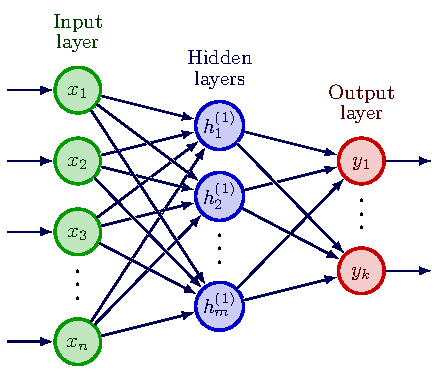
\includegraphics[width=\linewidth]{figures/nn}
        \caption{Typical "FeedForward" Neural Network Topology \cite{nn_diagram}}
        \label{fig:nn}
    \end{minipage}\hfill
    \begin{minipage}{0.48\textwidth}
        \centering
        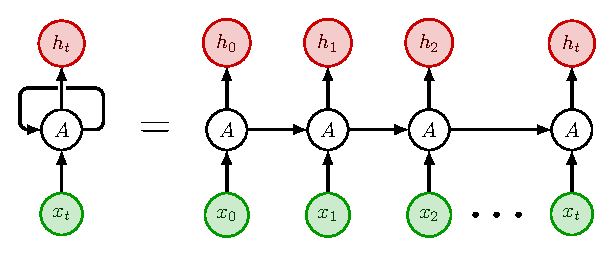
\includegraphics[width=\linewidth]{figures/rnn}
        \caption{Recurrent Neural Network (RNN) Topology \cite{rnn_diagram}}
        \label{fig:rnn}
    \end{minipage}
\end{figure*}

A machine learning model was developed to predict stock prices using article data and sentiment features. The literature review conducted concluded that while support vector machines (SVMs) are the most popular in the literature \cite{al_literature_review}, they often underperform in financial contexts due to their sensitivity to parameter tuning \cite{al_literature_review,zhang_markov_model}. \Cref{fig:nn,fig:rnn} illustrate the architectures of a typical feedforward neural network and a recurrent neural network (RNN), respectively. RNNs are designed for time series tasks and are thus well suited for stock prediction. RNNs, while powerful, have difficulties with 'memory' due to the number of layers after multiple recursions. Long Short Term Memory networks (LSTMs), a class of RNNs, address this by introducing memory cells with input, output, and forget gates, enabling more effective retention of information across time \cite{lstm_paper,ko_lstm}. Literature in this domain has demonstrated that LSTM models trained on both timeseries price data and sentiment analysis outperform models using price data alone \cite{heiden_lstm,ko_lstm}. 

\Cref{code:ml_single_stock} contains the source code for the single stock LSTM prediction code. Model training was performed in a Google Colab environent \cite{googlecolab}, due to the increased computational resources made available. Finance data was sourced from Yahoo Finance and merged with pre-collected sentiment data to form a unified dataframe, where each row corresponds to a single trading day, and days with no articles for that particular stock have sentiments set to a default 0 value. Three datasets were constructed: (1) a control set with only historical price data, (2) price data with VADER sentiment scores, and (3) price data with BERT sentiment embeddings. RNNs are trained using sliding windows of past data, so the model learns patterns by looking at every possible sequence of recent days.

Due to class imbalance—particularly the over-representation of mining stocks—no combined model across all stocks was trained. Instead, a separate model was trained for each stock. This approach better captures individual time series characteristics, such as company size, industry dynamics, and news volume. It also inherantly generalises well to other data sources (say, for other markets). While this method increases training time/computational cost, it allows for per-stock tuning and aligns with the approach taken by Heiden \cite{heiden_lstm}.

\lstinputlisting[language=Python, caption=Single stock prediction source code exract (full source code in \cref{code:ml_single_stock_full}), label=code:ml_single_stock]{../code/report_code_chunks/ml_single_stock_snippet.py}



A function, \code{train_test_split()}, was defined to segment each dataset into training and testing partitions. For training, a function \code{create_lstm_model(input_shape)} was defined to initialise and compile an LSTM model. The model consists of two stacked LSTM layers followed by a dense output layer, and was trained independently on each of the three datasets.
The LSTM architecture and training utilised the following hyperparameters:
\begin{itemize}
    \item Optimiser: Adam \((\alpha = 0.001,\ \beta_1 = 0.9,\ \beta_2 = 0.999,\ \epsilon = 1 \times 10^{-7})\)
\end{itemize}

These hyperparameters were chosen based on similar implmentations across online sources \cite{hyperparameters,rnn_example,adam_keras_api_docs}. The Adam optimiser was used due to it being "computationally efficient, having little memory requirement... and is well suited for problems that are large in terms of data/parameters" \cite{adam_keras_api_docs,adam_paper}, in addition to being prevalent in existing online implementations \cite{rnn_example}.

The model architecture consisted of two LSTM layers: the first with 64 units and \texttt{tanh} activation, returning sequences; the second with 32 units, also using \texttt{tanh}. These layer sizes were based on the model structure presented by Heiden \cite{heiden_lstm}. A final dense output layer with a single neuron used \texttt{tanh} activation, rather than the paper's \texttt{relu} due to inconsistent convergence during model training. The model was trained using the mean squared error loss function with a batch size of 64, which have been shown to be suitable for LSTMS \cite{hyperparameters,rnn_example}. 

Rather than training for a fixed number of epochs, early stopping was used to halt training if validation loss did not improve for 10 consecutive epochs, reducing the risk of overfitting. The training data was internally split 70/30 for training and validation, with the remaining 30\% of the original data reserved for final testing. Models were trained to minimise validation loss, ensuring generalisation to unseen data. 

Model performance was compared across the three datasets—the control model, VADER model, and BERT model—to assess the impact of sentiment features on predictive accuracy. Training loss, shown in \cref{fig:training_loss}, shows that all models converge, though models using sentiment features took longer, presumably due to the larger input dimentionality.

\begin{figure}[htbp]
    \centering
    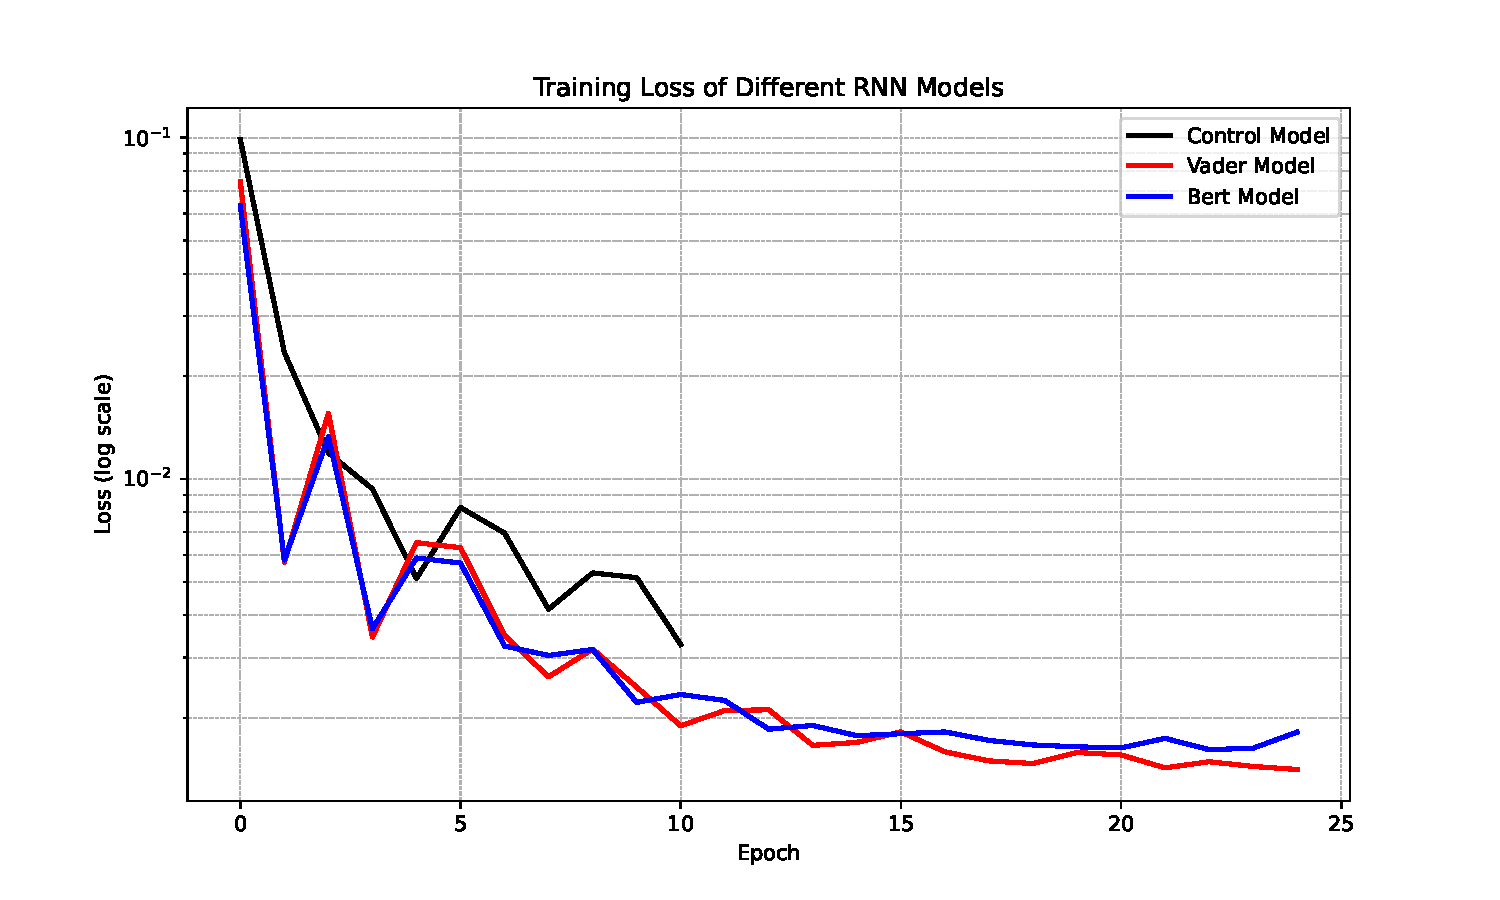
\includegraphics[width=0.5\textwidth]{figures/RAD_model_training_loss.pdf}
    \caption{Training loss vs. epoch plot for the LSTM model example}
    \label{fig:training_loss}
\end{figure}

\begin{figure}[htbp]
    \centering
    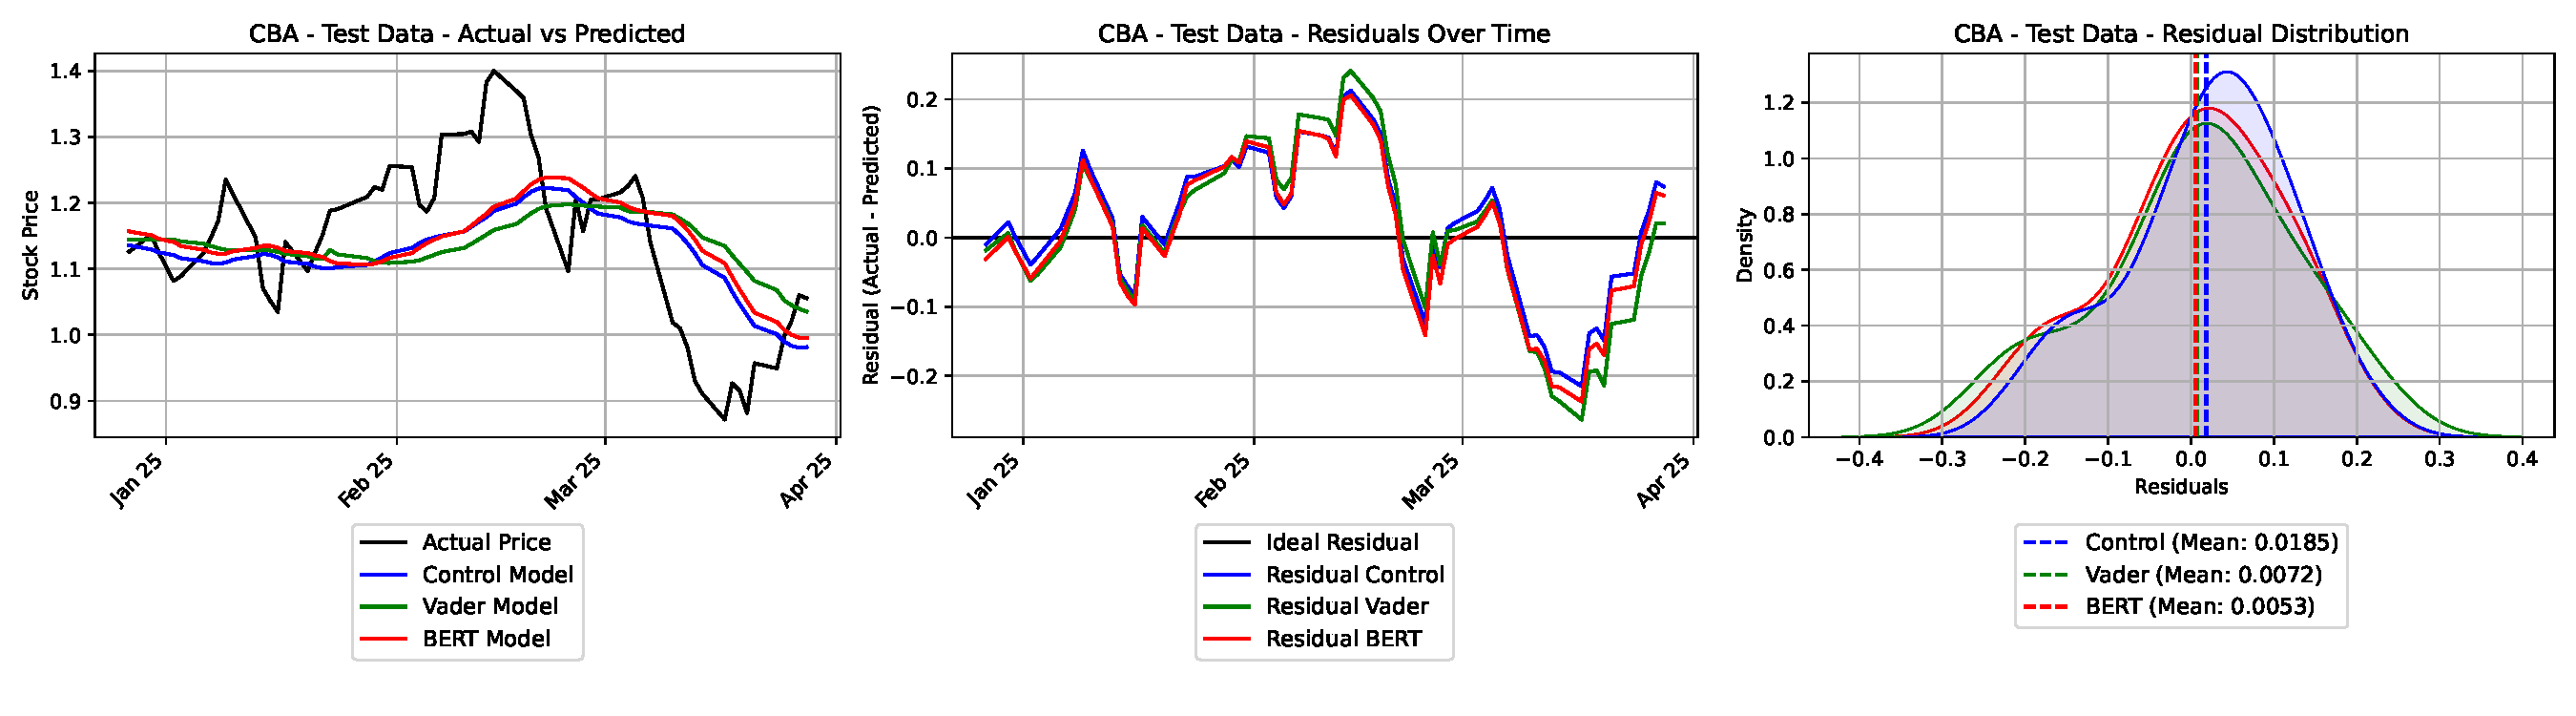
\includegraphics[width=\linewidth]{figures/residuals_CBA.pdf}
    \caption{Model Performance of CBA (Commonwealth Bank) LSTM model}
    \label{fig:model_performance_cba}
\end{figure}

\begin{table}[htbp]
    \centering
    \begin{tabular}{lccccc}
        \toprule
        \textbf{Model} & \textbf{BGD (Mining)} & \textbf{BOE (Energy)} & \textbf{CBA (Banking)} & \textbf{PIL (Tech)} & \textbf{RAD (Healthcare)} \\
        \midrule
        Control & 0.010008 & 0.006988 & 0.010436 & 0.018697 & 0.001870 \\
        Vader   & 0.016969 & 0.006399 & 0.014232 & 0.005896 & 0.001202 \\
        BERT    & 0.017634 & 0.006984 & 0.011358 & 0.015211 & 0.001345 \\
        \bottomrule
    \end{tabular}
    \caption{MSE computed across selected stocks and sectors (lower is better).}
    \label{tab:single_stock_performance}
\end{table}



\Cref{fig:model_performance_cba} shows the model performance of the LSTM model trained on the CBA (Commonwealth Bank) data, a typical result seen across multiple stocks. It can be seen that the trend each of these models exhibit are highly correlated, even despite their difference in input features, and that both the time series trend and the overall distribution of their residuals have close resemblance to each other. \Cref{tab:single_stock_performance} shows a complete summary of the stock codes tested with the LSTM method. It is evident that the incorperating sentiment data is seen to decrease the performance of the model in the case of BGD, CBA; and improves the performance in the case of BOE, PIL, and RAD, with VADER models having a lower MSE. 

This demonstrates that sentiment data does not meaningfully improve the predictive performance of the model. This performance may be largely due to the sparsity of news coverage per stock. As shown in \Cref{fig:stock_code_distribution}, even the most frequently mentioned stock, \textit{ASX:BGD}, appeared in only 40 articles over a 16-month period—equating to just 2.5 articles per month. Such sparsity undermines the reliability and sustainability of sentiment-driven predictive models, a challenge also identified in literature \cite{zhang_markov_model}. One solution to the sparsity would be to create synthetic data, which would not be a true representation of prices reflecting real information. As mentioned previously, no domain on the internet meets all the criteria for a suitable data source, so supplementing the article corpus from articles from another website was not a feasible solution, at least within the context of Australian market.

A solution to the data sparsity was posited, to predict the broader ASX200 index and verify if sparsity was the reason for the poor predictive performance of the sentiment. This shift not only mitigates the sparsity issue but also allows the model to capture macroeconomic sentiment and general political news, which are more consistently reported and likely to influence overall market trends (use articles with no stock codes listed).

Performing a similar analysis on the asx200 index (\cref{code:ml_asx200}) and incorperating articles that are in SmallCaps' 'hot topics' category (which is general news that pertains to no industry in particular), and also mention stocks within the ASX200. This way, we can include general politics and other news that may affect the index as a whole. \Cref{fig:asx200_article_count} shows the article count for the ASX200 index, showing that the problem of sentiment sparsity is no longer an issue, and days with multiple articles can have their sentiments averaged. \Cref{fig:asx200_loss_epoch} shows the training loss vs. epoch plot for the ASX200 model, showing that model convergence occours at the around the 40-50th epoch for all three models. \Cref{fig:asx200_model_performance} shows the model performance of the ASX200 index models, showing again that the models have similar trends, and that the introduction of sentiments from \textit{SmallCaps} articles does not meaningfully improve the performance of the model, contributing to similar, if not worse performance, as seen with the time series, and overall distribution of the residual (\cref{fig:asx200_model_performance}) and the numeric results (\cref{tab:asx200_model_performance}). 


\begin{figure*}[htbp]
    \centering
    \begin{minipage}{0.48\textwidth}
        \centering
        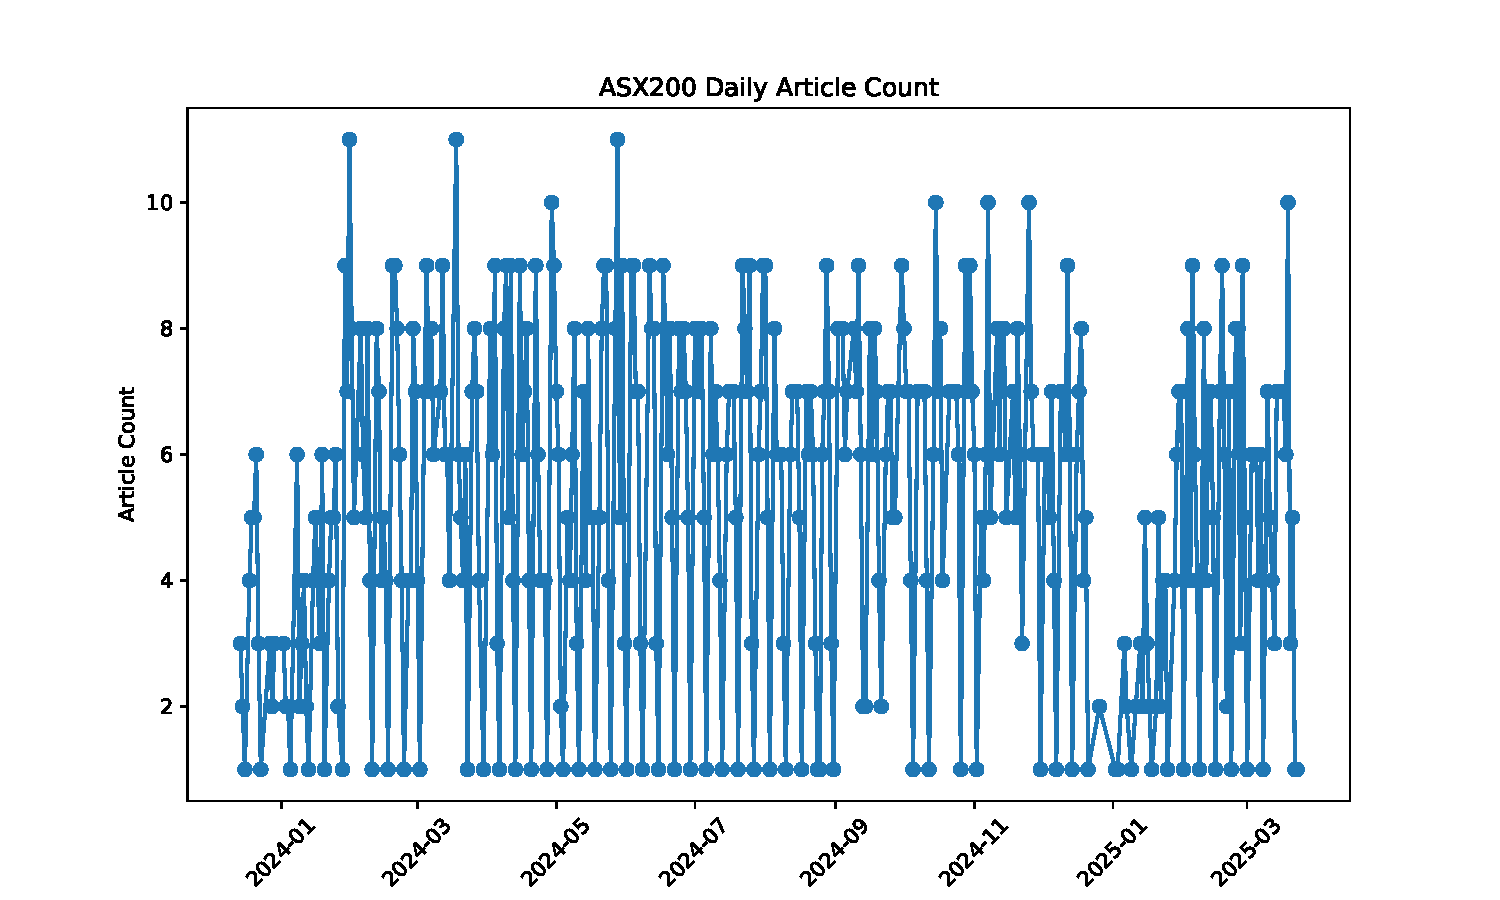
\includegraphics[width=\linewidth]{figures/asx200_article_count.pdf}
        \caption{Article count for the ASX200 index} 
        \label{fig:asx200_article_count}
    \end{minipage}\hfill
    \begin{minipage}{0.48\textwidth}
        \centering
        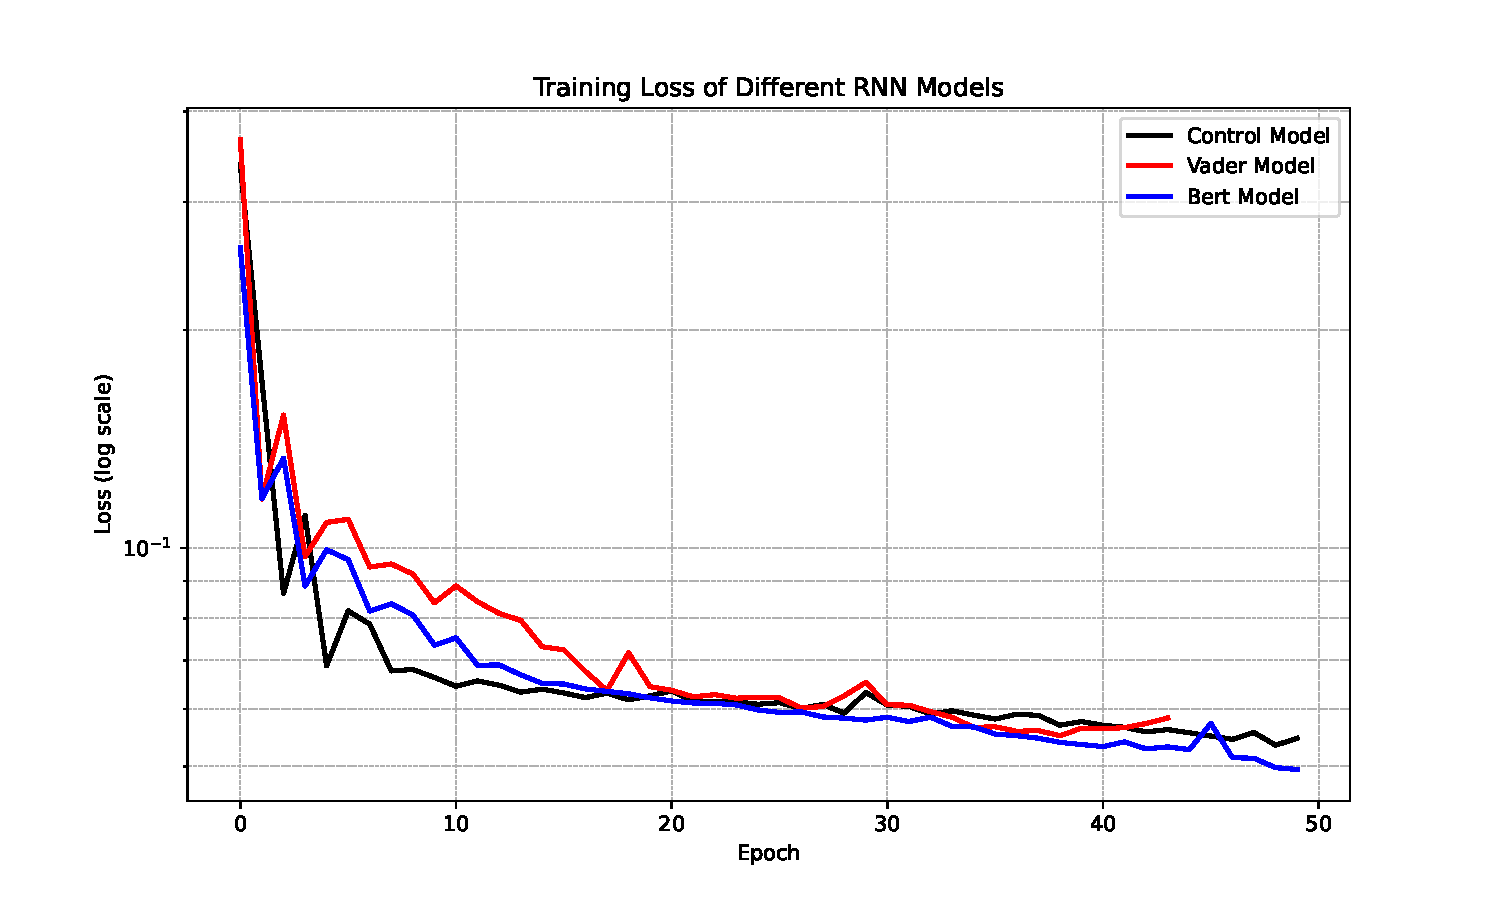
\includegraphics[width=\linewidth]{figures/ASX200_model_training_loss.pdf}
        \caption{Training loss vs. epoch plot for ASX200 model}
        \label{fig:asx200_loss_epoch}
    \end{minipage}
\end{figure*}

\begin{figure}[htbp]
    \centering
    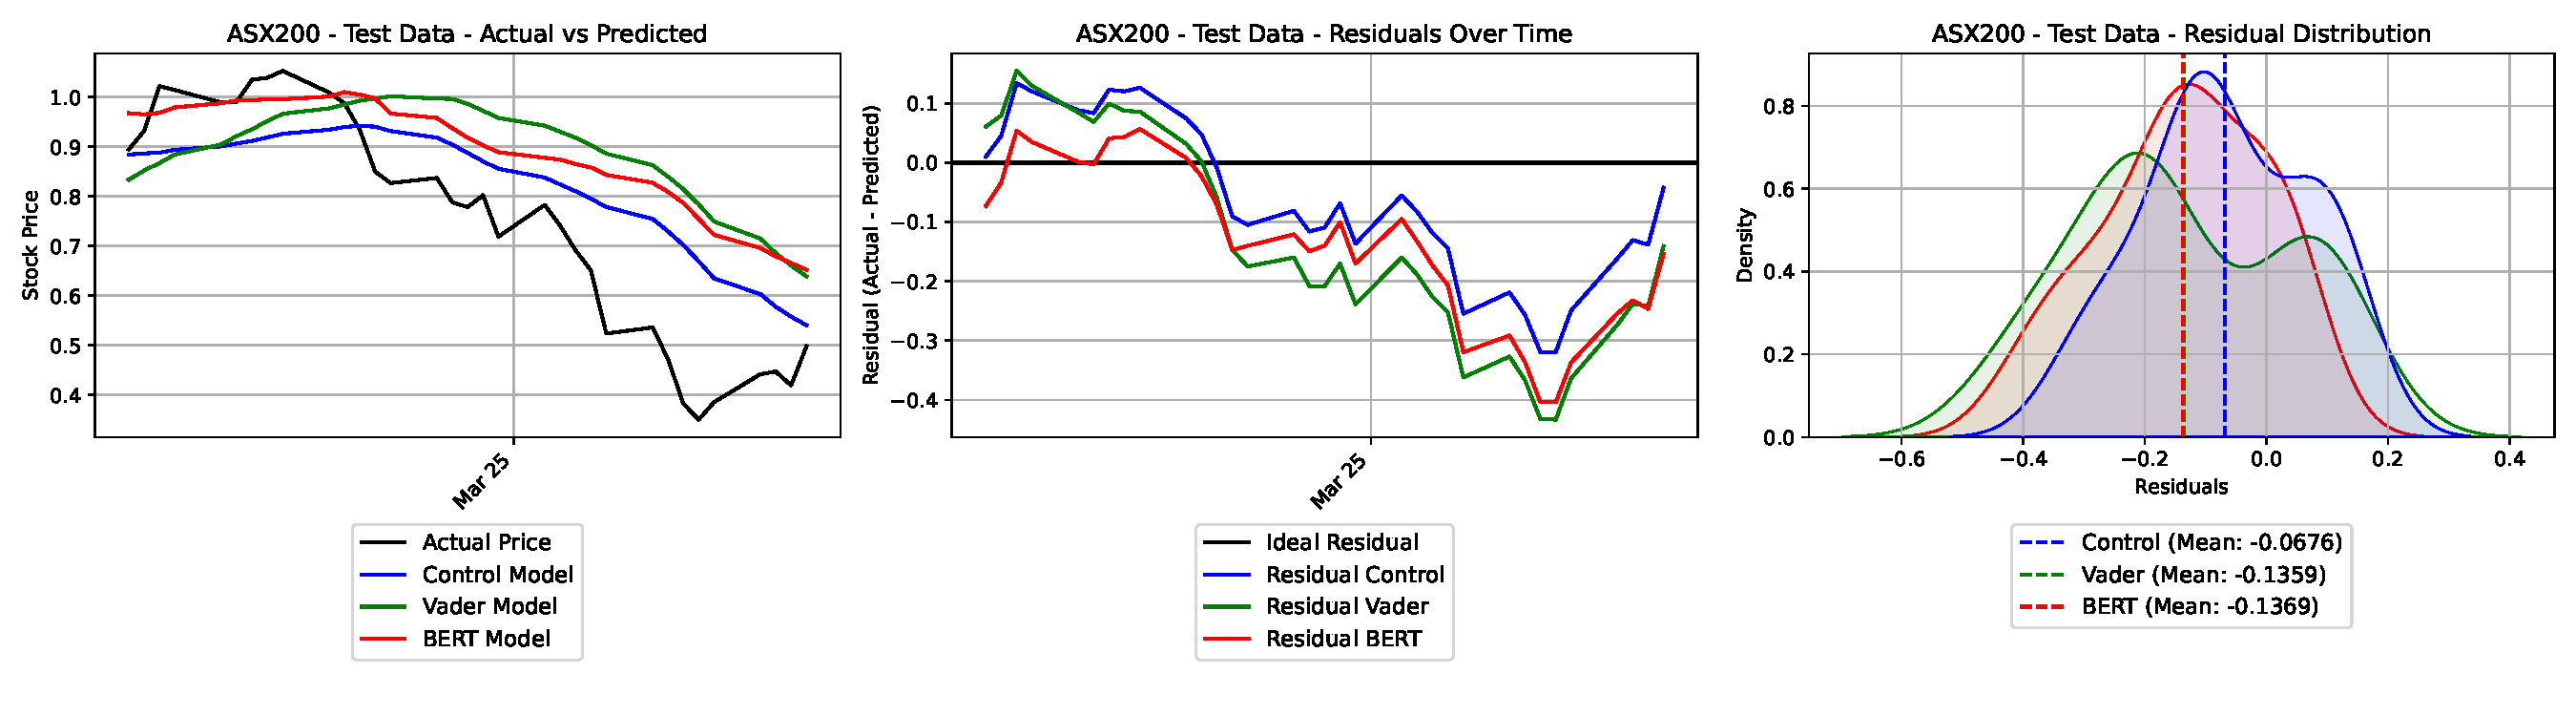
\includegraphics[width=\linewidth]{figures/residuals_ASX200.pdf}
    \caption{Model Performance of ASX200 Index Model}
    \label{fig:asx200_model_performance}
\end{figure}

\begin{table}[h]
    \centering
    \caption{Model performance metrics for ASX200}
    \label{tab:asx200_model_performance}
    \begin{tabular}{lccc}
    \toprule
    \textbf{Model} & \textbf{MSE} & \textbf{RMSE} & \textbf{MAE} \\
    \midrule
    Control & 0.022140 & 0.148794 & 0.126688 \\
    VADER   & 0.048714 & 0.220713 & 0.189641 \\
    BERT    & 0.036432 & 0.190871 & 0.151437 \\
    \bottomrule
    \end{tabular}
\end{table}
    
    



